\documentclass[aspectratio=169,
				xcolor=table]{beamer}
				
% Load general definitions
\usepackage[utf8]{inputenc}
%\usepackage[T1]{fontenc}
\usepackage[brazil]{babel}
\usepackage{amsmath}
\usepackage{amsfonts}
\usepackage{amssymb}
\usepackage{graphicx}
\usepackage{verbatim}
\usepackage{cancel}
\usepackage{askmaps}
\usepackage{tabularx}
\usepackage[table]{xcolor}
%\usepackage{tikz}
\usepackage{multirow}
\usepackage{mathtools}
\usepackage{color, colortbl}
\usepackage{etoolbox}
\usepackage{pbox}
\usepackage{changepage}
\usepackage{xpatch}
\usepackage{array}
\usepackage{marvosym}
\usepackage{tabu}
\usepackage{multicol}
\usepackage{listings}
\usepackage{underscore}
\usepackage{filecontents}
\usepackage[]{algorithm2e}
\usepackage{ragged2e}

\newcolumntype{P}[1]{>{\centering\arraybackslash}m{#1}}
\definecolor{Gray}{gray}{0.75}
\definecolor{Gray2}{gray}{0.85}

\definecolor{lightBlue}{HTML}{DAE8FC}
\definecolor{Blue}{RGB}{51, 51, 204}

%\useinnertheme[lily]{rounded}
\usetheme{UniEvangelica}
%\usetheme{Copenhagen}
%\usetheme{Berlin}
%\usecolortheme{dolphin}
\tolerance=1
\emergencystretch=\maxdimen
\hyphenpenalty=10000
\hbadness=10000

\setbeamertemplate{navigation symbols}{}%remove navigation symbols


\let\olditem=\item% 
\renewcommand{\item}{\olditem \justifying}%
\def\center{\trivlist \centering\item\relax}
\def\endcenter{\endtrivlist}

\setbeamertemplate{itemize/enumerate body begin}{\large}
\setbeamertemplate{itemize/enumerate subbody begin}{\large}

\setbeamertemplate{itemize item}{\raisebox{0.1ex}{$\blacktriangleright$}\hskip0.1em}
\setbeamertemplate{itemize subitem}{\raisebox{0.1ex}{$\blacktriangleright$}\hskip0.1em}

\newcommand{\greenarrow}{\textcolor{green}{\rotatebox[origin=c]{180}{\MVArrowDown}}}

\newcommand{\redarrow}{\textcolor{red}{\MVArrowDown}}

%\newcommand{\ftable}{
%	\begin{table}
%		\large
%		\centering
%		\rowcolors{1}{\ifnumless{\rownum}{2}{Blue}{lightBlue}}{}
%}

\newenvironment{eftable}{
	\begin{table}
		\large
		\centering
		\rowcolors{1}{}{Blue}
		\rowcolors{1}{\ifnumless{\rownum}{2}{Blue}{lightBlue}}{}
	}
	{
	\end{table}
}


%\setbeamertemplate{frametitle}
%{
%	%\vspace*{-2em}	
%	\insertframetitle
%
%	 %\textcolor{white}{\LARGE \insertframetitle}
%
%}

% Specific definitions
\institute[]{\uppercase{Engenharia de Software}}
\title[]{Arquitetura e Organização de Computadores}
\subtitle[]{\uppercase{Memória Secundária}}
\author[]{Prof. Alexandre Tannus}
\date{}

\AtBeginSection{\frame{\tableofcontents[currentsection]}}

\begin{document}
	\setbeamertemplate{caption}{\raggedright\insertcaption\par}

	\begin{frame}
		\titlepage
	\end{frame}
	
	\begin{frame}{Objetivos}
		\begin{itemize}
			\item Recordar a hierarquia de memórias
			\vspace{1em}
			\item Relatar a evolução da memória secundária
			\vspace{1em} 
			\item Distinguir entre meios magnéticos, óticos e eletrônicos de armazenamento
		\end{itemize}
	\end{frame}

	\begin{frame}{Metodologia}
		\begin{itemize}
			\item O tema da aula é exposto pelo professor em sala de aula. Os alunos interagem durante a apresentação para resolução de dúvidas e exposição de questionamentos relevantes ao tema, os quais podem ser sanados diretamente pelo professor ou serem colocados em discussão pela turma. 
			\vspace{1em}
			\item Ao final da exposição do conteúdo são resolvidos exercícios de fixação, para melhor compreensão do tema. As questões podem ser retiradas de concursos públicos, ENADE, POSCOMP ou de autoria do próprio professor.
		\end{itemize}
	\end{frame}

	\begin{frame}
		\tableofcontents		
	\end{frame}	
	
	\section{Introdução}
	
		\begin{frame}{Hierarquia de memória}
			\begin{figure}[hbtp]
				\centering
				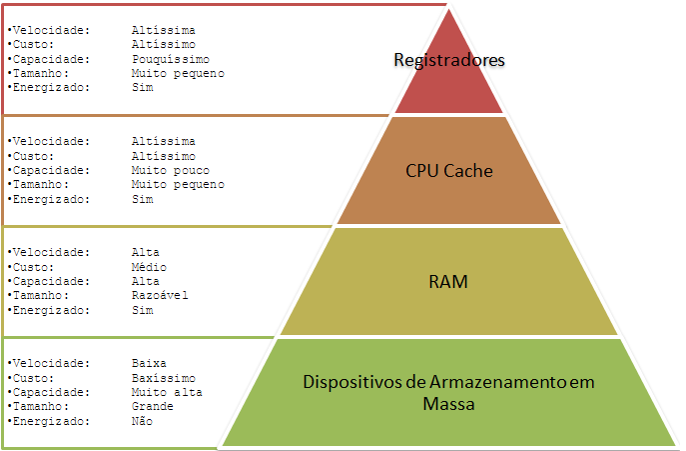
\includegraphics[height=0.8\textheight, keepaspectratio]{../figs/cap07/memoria.png}
			\end{figure}
		\end{frame}
		
		\begin{frame}{Tecnologias de memória}
			\begin{columns}
				\begin{column}{0.5\textwidth}
					\begin{itemize}
						\item Semicondutores 
						\begin{itemize}
							\item SSD
						\end{itemize}
						\vspace{1em}
						\item Magnética
						\begin{itemize}
							\item HD, disquete
						\end{itemize}
						\vspace{1em}
						\item Ótica
						\begin{itemize}
							\item CD, DVD
						\end{itemize}
					\end{itemize}
				\end{column}
				\begin{column}{0.5\textwidth}
					\begin{figure}[hbtp]
					\centering
					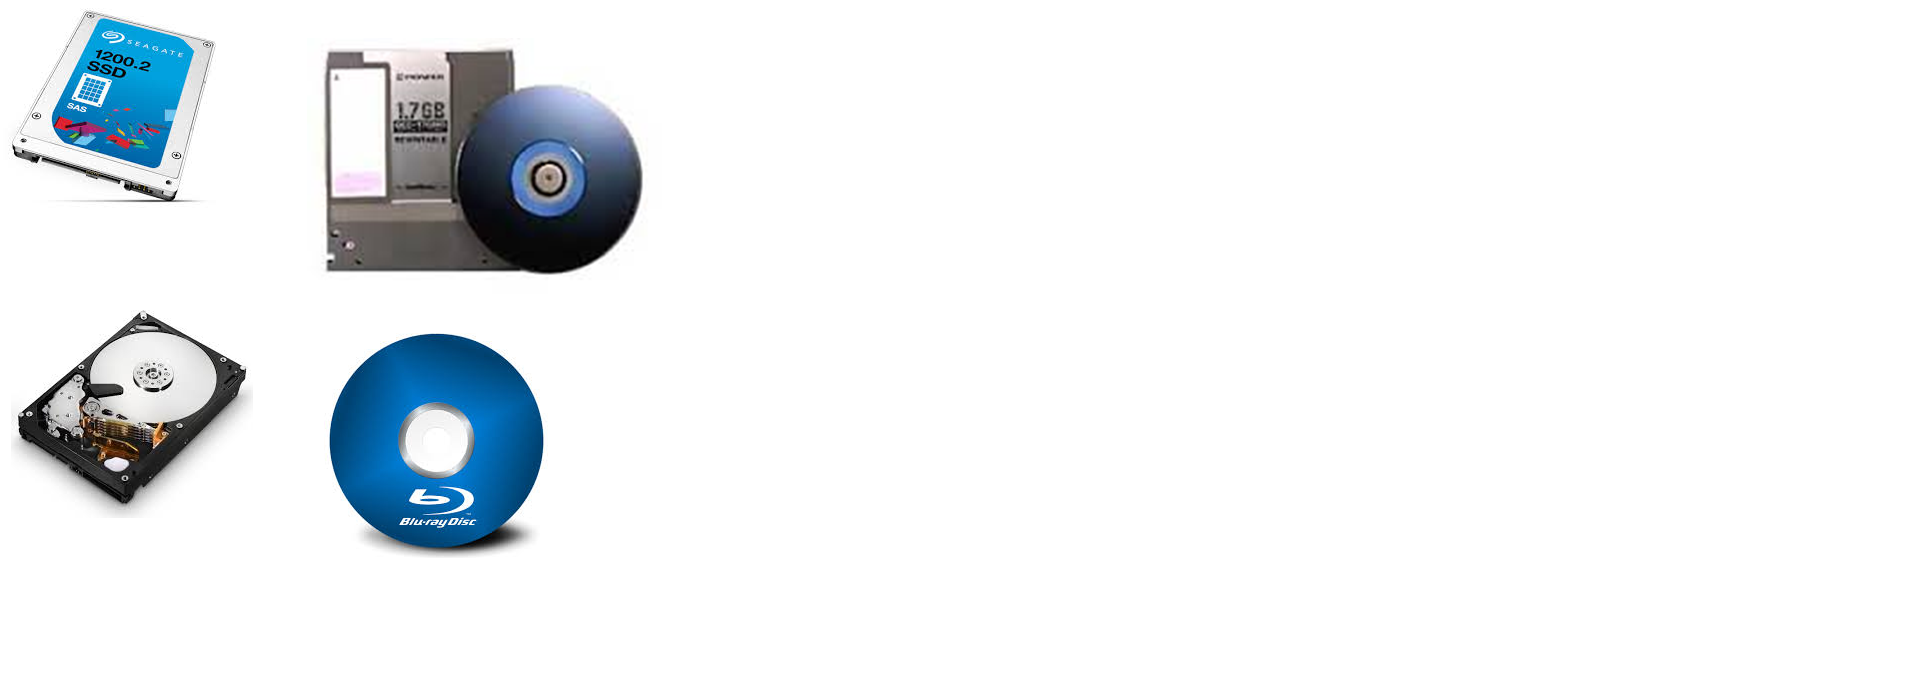
\includegraphics[height=0.85\textheight, keepaspectratio]{../figs/cap08/massa.png}
					\end{figure}
					
				\end{column}
			\end{columns}
		\end{frame}		
	
		\begin{frame}{Hierarquia de armazenamento}
			\begin{eftable}				\centering
				\begin{tabular}{ll}
				{\color[HTML]{FFFFFF} Dispositivo} & {\color[HTML]{FFFFFF} Tempo de acesso} \\
				Registradores                      & $0,25 ns$                                \\
				Cache                              & $1-10 ns$                                \\
				Memória convencional               & $10-50 ns$                               \\
				Memória flash                      & $120 \mu s$                                 \\
				Disco magnético                    & $10-50 ms$                               \\
				Disco ótico                        & $100-500 ms$                             \\
				Fita magnética                     & $0,5 s$                    
				\end{tabular}
			\end{eftable}			
		\end{frame}	
		
		
	\section{Meios Magnéticos}
	
	\begin{frame}{Introdução}
		\begin{itemize}
			\item Principal meio de armazenamento em massa de um computador
			\vspace{1em}
			\item Capacidade atual na faixa de terbytes (TB)
			\begin{itemize}
				\item Dimensões micrométricas da cabeça de leitura/escrita
			\end{itemize}
			\vspace{1em}
			\item Tempo de acesso rápido (comparado a outros dispositivos de memória secundária)
			\begin{itemize}
				\item Alta rotação (3600 a 15000 rpm)			
			\end{itemize}
		\end{itemize}
	\end{frame}
	
	\begin{frame}{Evolução}
		\begin{columns}
			\begin{column}{0.5\textwidth}
				\begin{itemize}
					\item Fita Magnética
					\begin{itemize}
						\item Áudio (1928)
						\item Dados em computadores (1950) 
						\item Vídeo (1980)
						
					\vspace{1em}	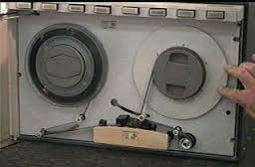
\includegraphics[width=0.65\textwidth, keepaspectratio]{../figs/cap08/fita01.png}
					\end{itemize}
				\end{itemize}
			\end{column}
			\begin{column}{0.5\textwidth}
				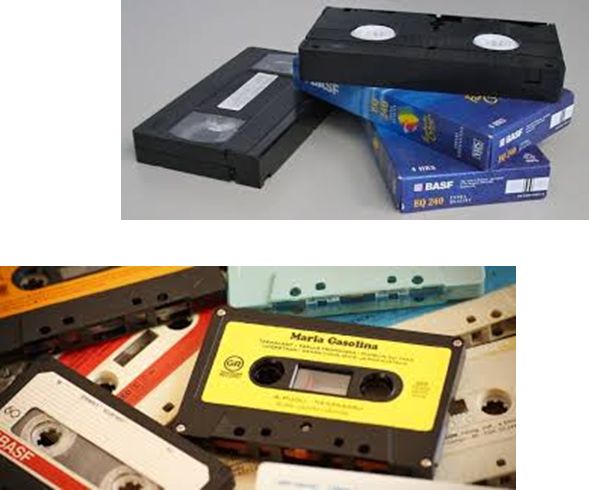
\includegraphics[height=0.7\textheight, keepaspectratio]{../figs/cap08/fita02.png}
			\end{column}
		\end{columns}
	\end{frame}
	
	\begin{frame}{Evolução}
		\begin{columns}
			\begin{column}{0.5\textwidth}
				\begin{itemize}
					\item Disquete (\textit{Floppy disks})
					\begin{itemize}
						\item Desenvolvido pela IBM (1971)
						\item Tamanhos variados
						\item Atualmente obsoleto
					\end{itemize}
				\end{itemize}
				\vspace{1em}
				
				\begin{figure}
					\centering				
					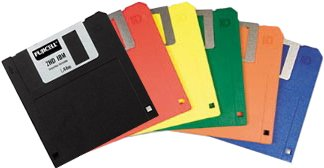
\includegraphics[width=0.75\textwidth, keepaspectratio]{../figs/cap08/disquete}
				\end{figure}
				
			\end{column}
			\begin{column}{0.5\textwidth}
			\vspace{-1.5em}
			\begin{eftable}
				\centering
				\begin{tabular}{ll}
				{\color[HTML]{FFFFFF} \begin{tabular}[c]{@{}l@{}}Tamanho \\ (polegada)\end{tabular}} & {\color[HTML]{FFFFFF} \begin{tabular}[c]{@{}l@{}}Capacidade (bytes)\end{tabular}} \\
				8                                                                                    & \begin{tabular}[c]{@{}l@{}}80 k,   256 k\\   800 k,   1 M\end{tabular}            \\
				5 $^1/_4$ & \begin{tabular}[c]{@{}l@{}}160 k ,   360 k\\   720 k ,   1.2 M\end{tabular}        \\
				3 $^1/_ 2$                                                                                & \begin{tabular}[c]{@{}l@{}}720 k ,   1.44 M\\   2.88 M ,   5.76 M\end{tabular}    
				\end{tabular}
			\end{eftable}			
					
			\end{column}
		\end{columns}
	\end{frame}
	
	\begin{frame}{\textit{Hard Disks} - HD}
		\begin{itemize}
			\item Dispositivo de armazenamento mais comum nos computadores atuais
			\vspace{1em}
			\item Capacidade de armazenamento em terabytes (TB)
			\vspace{1em}
			\item Custo/byte muito baixo

			\begin{figure}
				\centering
				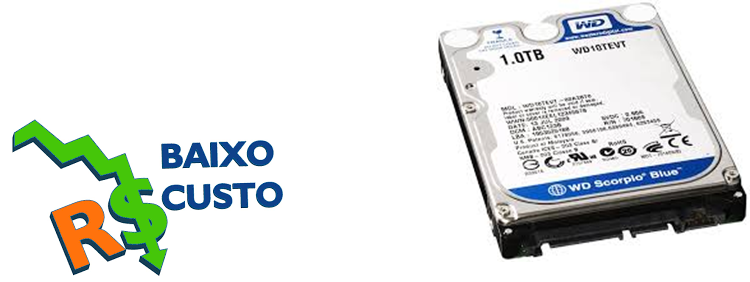
\includegraphics[width=0.6\textwidth, keepaspectratio]{../figs/cap08/hd01.png}
			\end{figure}

		\end{itemize}
	\end{frame}
	
	\begin{frame}{Construção}
		\begin{columns}
			\begin{column}{0.6\textwidth}
			\begin{itemize}
				\item Discos circulares de material não magnético
				\begin{itemize}
					\item Alumínio
					\item Liga de alumínio
					\item Vidro
				\end{itemize}

				\vspace{1em}
				\item Material magnetizável cobre o disco

			\end{itemize}
			
			\end{column}
			\begin{column}{0.4\textwidth}
							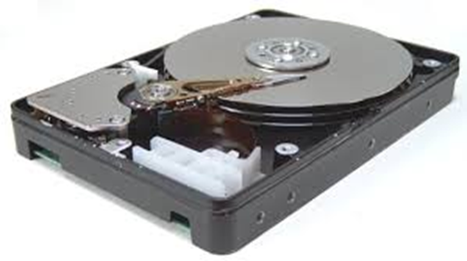
\includegraphics[width=0.9\textwidth, keepaspectratio]{../figs/cap08/hd02.png}

			\end{column}
		\end{columns}
	\end{frame}
	
	\begin{frame}{Construção}
		\begin{figure}
		\centering
		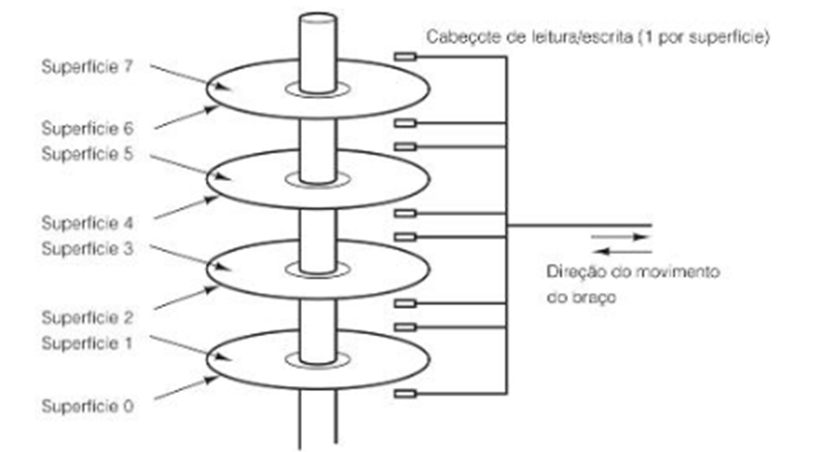
\includegraphics[height=0.8\textheight, keepaspectratio]{../figs/cap08/hd03.png}
		\end{figure}			
	\end{frame}
	
	\begin{frame}{Construção}
		\begin{figure}
		\centering
		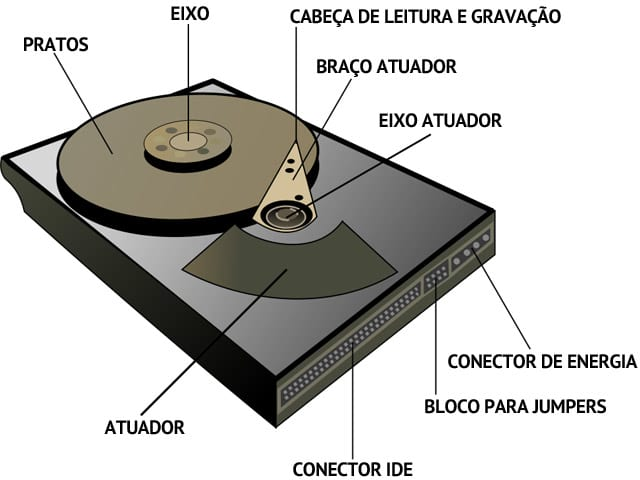
\includegraphics[height=0.8\textheight, keepaspectratio]{../figs/cap08/hd04}
		\end{figure}			
	\end{frame}

	\begin{frame}{Construção}
		\begin{figure}
		\centering
		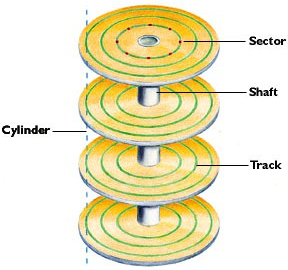
\includegraphics[height=0.8\textheight, keepaspectratio]{../figs/cap08/hd05}
		\end{figure}			
	\end{frame}
	
	\begin{frame}{Tempo de acesso}
		\begin{itemize}
			\item Tempo de busca (\textit{seek time})
			\begin{itemize}
				\item Tempo de alinhamento da cabeça de leitura/gravação com o cilindro contendo a trilha com o setor desejado
			\end{itemize}
			\vspace{1em}
			\item Latência de rotação (\textit{rotation delay})
			\begin{itemize}
				\item Tempo para o disco rodar até a posição de início dos dados no setor
			\end{itemize}
			\vspace{1em}
			\item Tempo de transferência de dados (\textit{transfer time})
		\end{itemize}
	\end{frame}
	
	\begin{frame}{Tempo de acesso}
		\begin{figure}
		\centering
		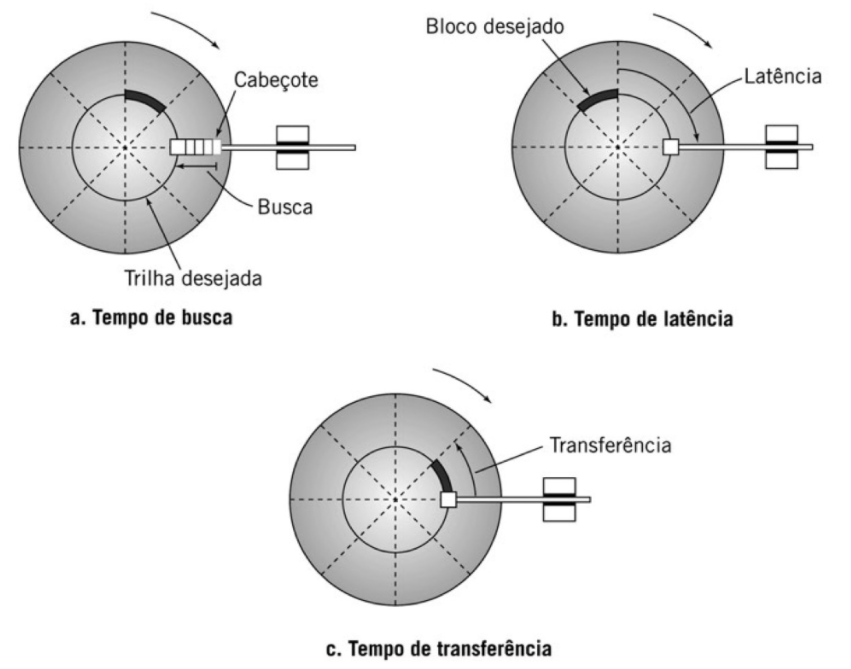
\includegraphics[height=0.8\textheight, keepaspectratio]{../figs/cap08/disktime}
		\end{figure}			
	\end{frame}
	
	\begin{frame}{Capacidade do disco}
		\begin{itemize}
			\item Superfícies (s)
			\item Trilhas por superfície (tps)
			\item Setores por trilha (spt)
			\item Bytes por setor (bps)
			
			\begin{equation*}
				\Huge
				capacidade = s * tps * spt * bps
			\end{equation*}
		\end{itemize}
	\end{frame}
	
	\begin{frame}{Organização dos dados}
		\begin{itemize}
			\item Gravação magnética em direções opostas
			\vspace{1em}
			\item Utilização de coidficação NRZ (\textit{non return to zero})
			\vspace{1em}
			\item Dados + setor + CRC (verificação de erros)
		\end{itemize}
	\end{frame}
	
	\begin{frame}{Organização dos dados}
		\begin{itemize}
			\item Minimizar tempos de busca e atraso de rotação
			\begin{itemize}
				\item Dados acessados em conjuntos colocados em cilindros adjacentes
			\end{itemize}
			\vspace{1em}
			\item Atribuição de setores lógicos adjacentes a setores físicos 
			\vspace{1em}
			\item Atividade realizada pelo controlador do disco
			\begin{itemize}
				\item Transparente para o usuário
			\end{itemize}
		\end{itemize}
	\end{frame}
	
	\begin{frame}{Matrizes de discos}
		\begin{itemize}
			\item RAID (\textit{Redundant Array of Independent Disks})
			\begin{itemize}
				\item Arranjo de discos que trabalham em conjunto
			\end{itemize}
			\item Aumento da capacidade de armazenamento
			\vspace{1em}
			\item Aumento da disponibilidade
			\vspace{1em}
			\item Aumento da segurança
		\end{itemize}
	\end{frame}
	
	\begin{frame}[t]{RAID (\textit{Redundant Array of Independent Disks})}{Níveis}	
		\begin{columns}[t]
			\begin{column}{0.5\textwidth}
				\begin{itemize}
					\item RAID 0
					\begin{itemize}
						\item Múltiplos discos
						\item Nenhuma redundância
					\end{itemize}
				\end{itemize}				
			\end{column}
			\begin{column}{0.5\textwidth}							
				\begin{figure}
					\centering
					\vspace{-1em}
					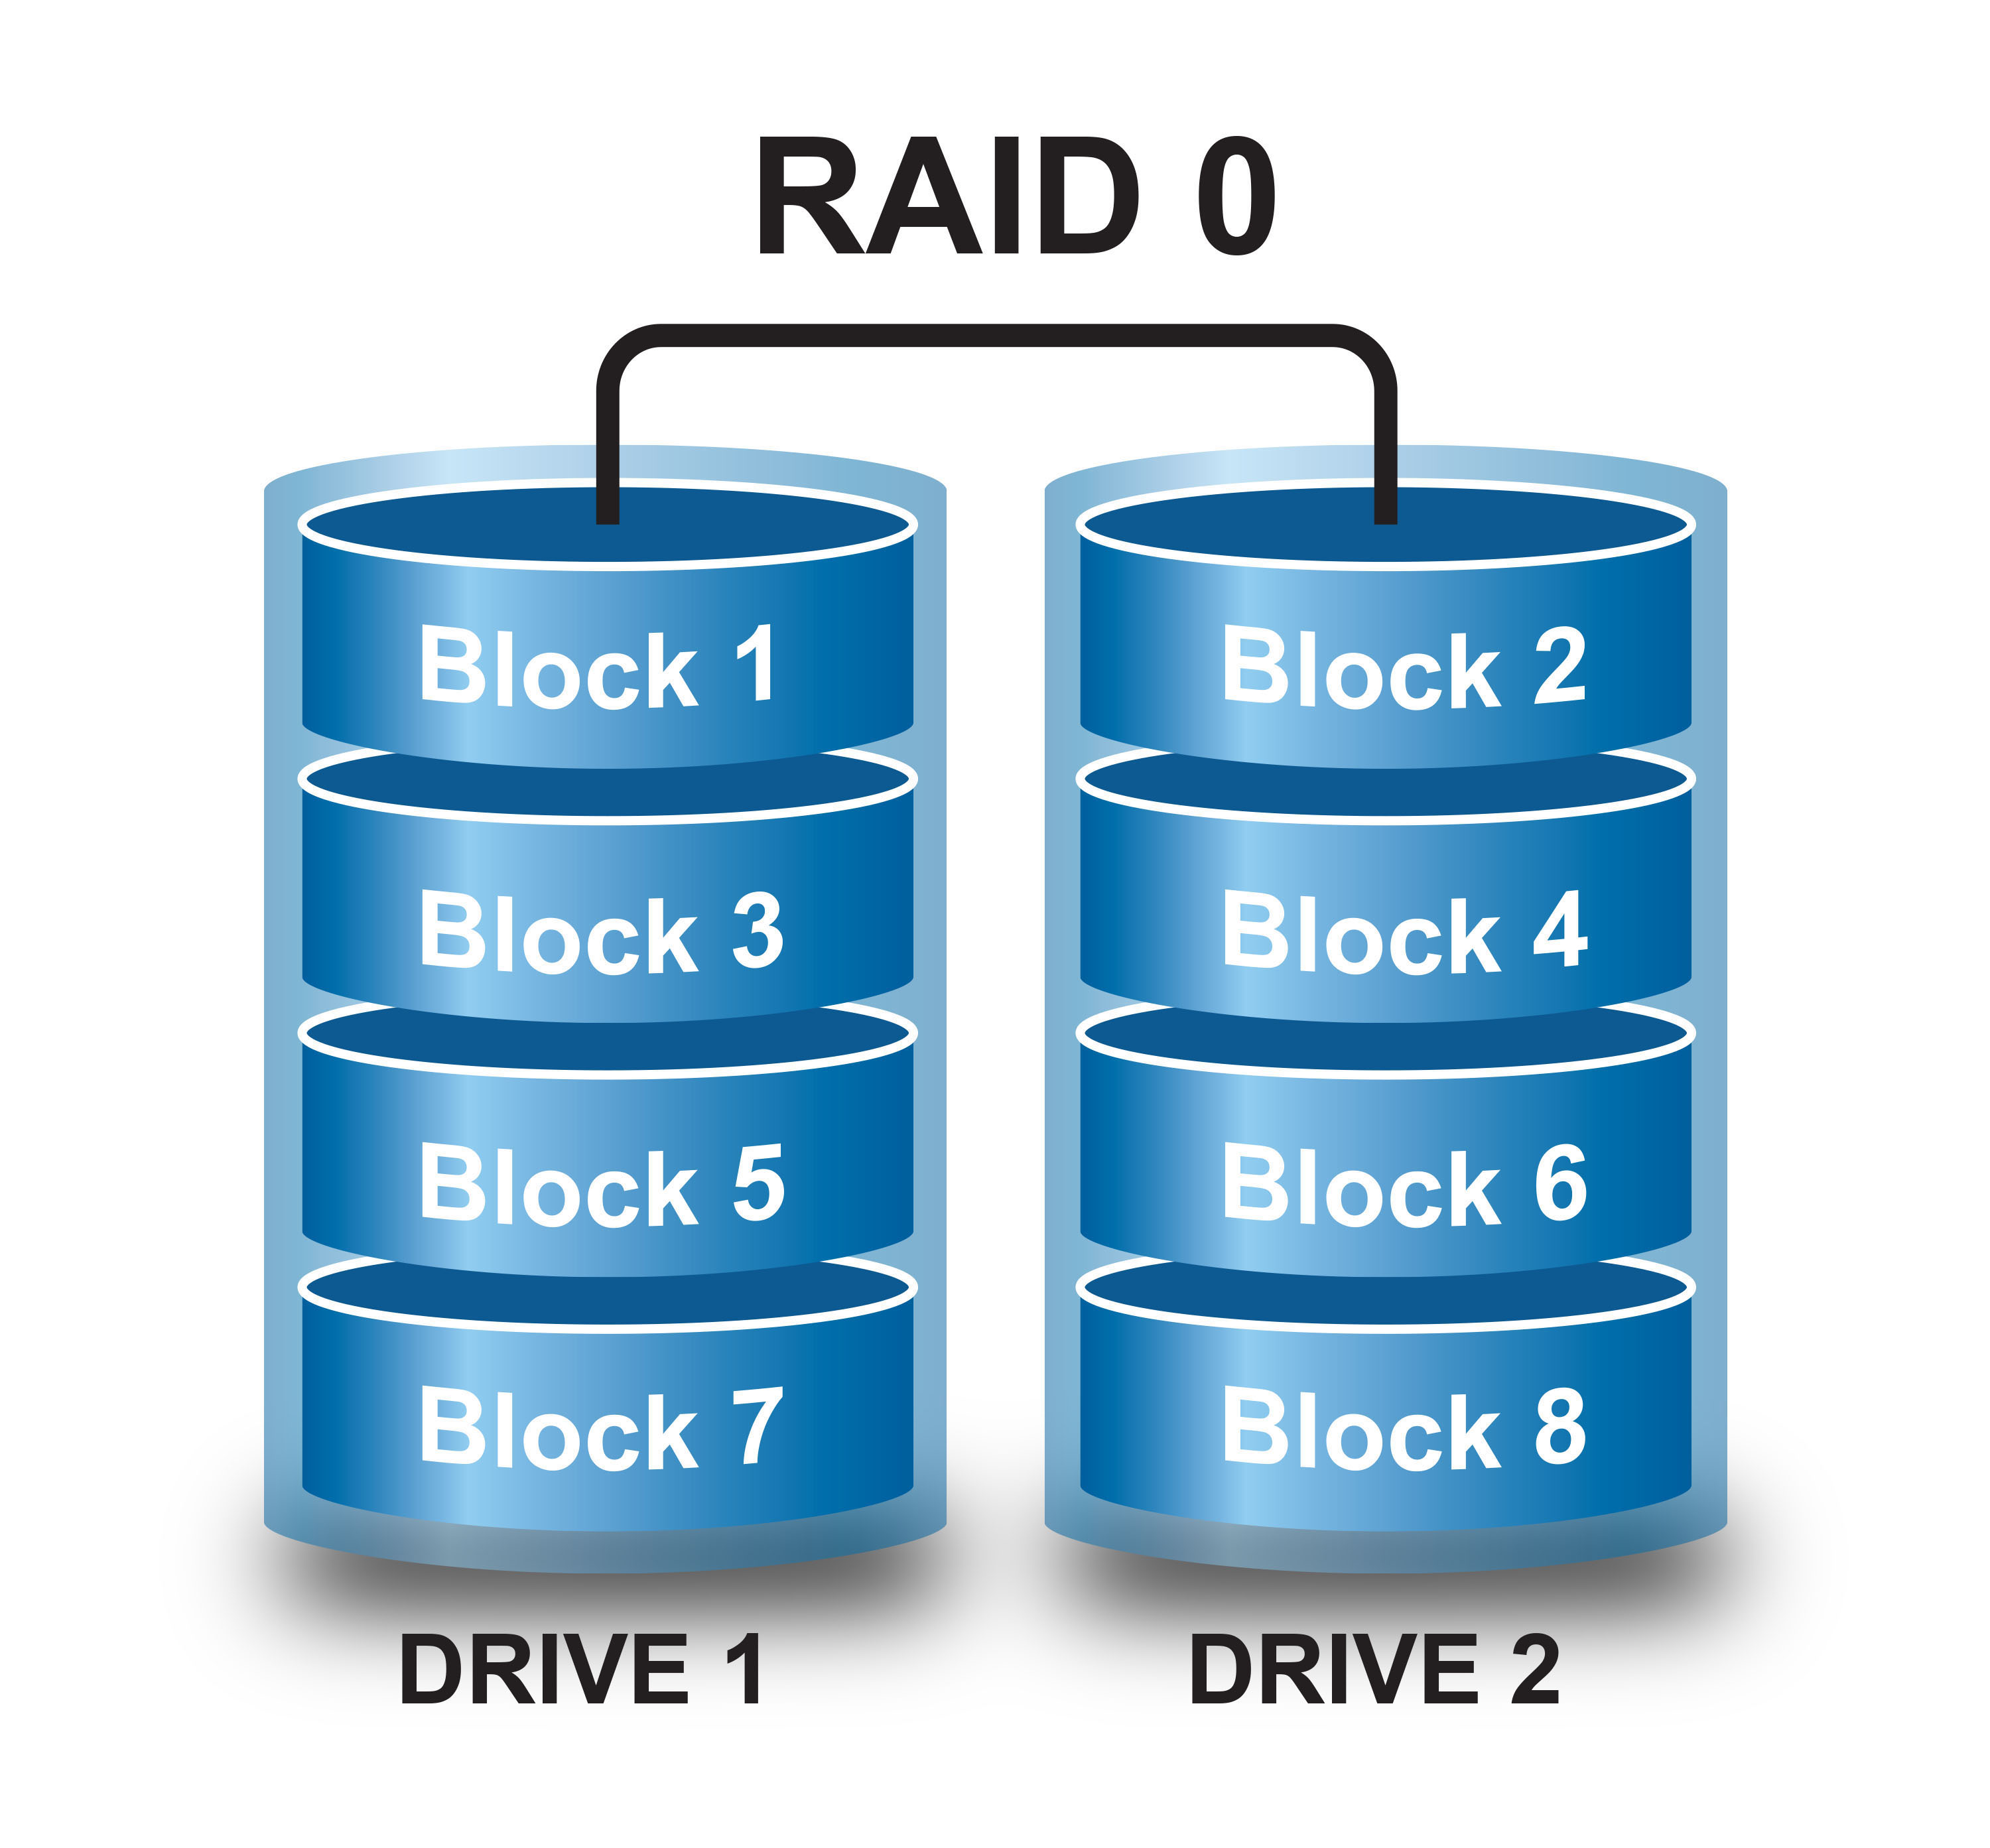
\includegraphics[height=0.7\textheight, keepaspectratio]{../figs/cap08/raid0}
				\end{figure}
			\end{column}
		\end{columns}

		
	\end{frame}
	
	\begin{frame}[t]{RAID (\textit{Redundant Array of Independent Disks})}{Níveis}	
		\begin{columns}[t]
			\begin{column}{0.5\textwidth}
				\begin{itemize}
					\item RAID 1
					\begin{itemize}
						\item Espelhamento de discos
					\end{itemize}
				\end{itemize}
				
			\end{column}
			\begin{column}{0.5\textwidth}				
				\begin{figure}
					\centering
				\vspace{-1em}	
					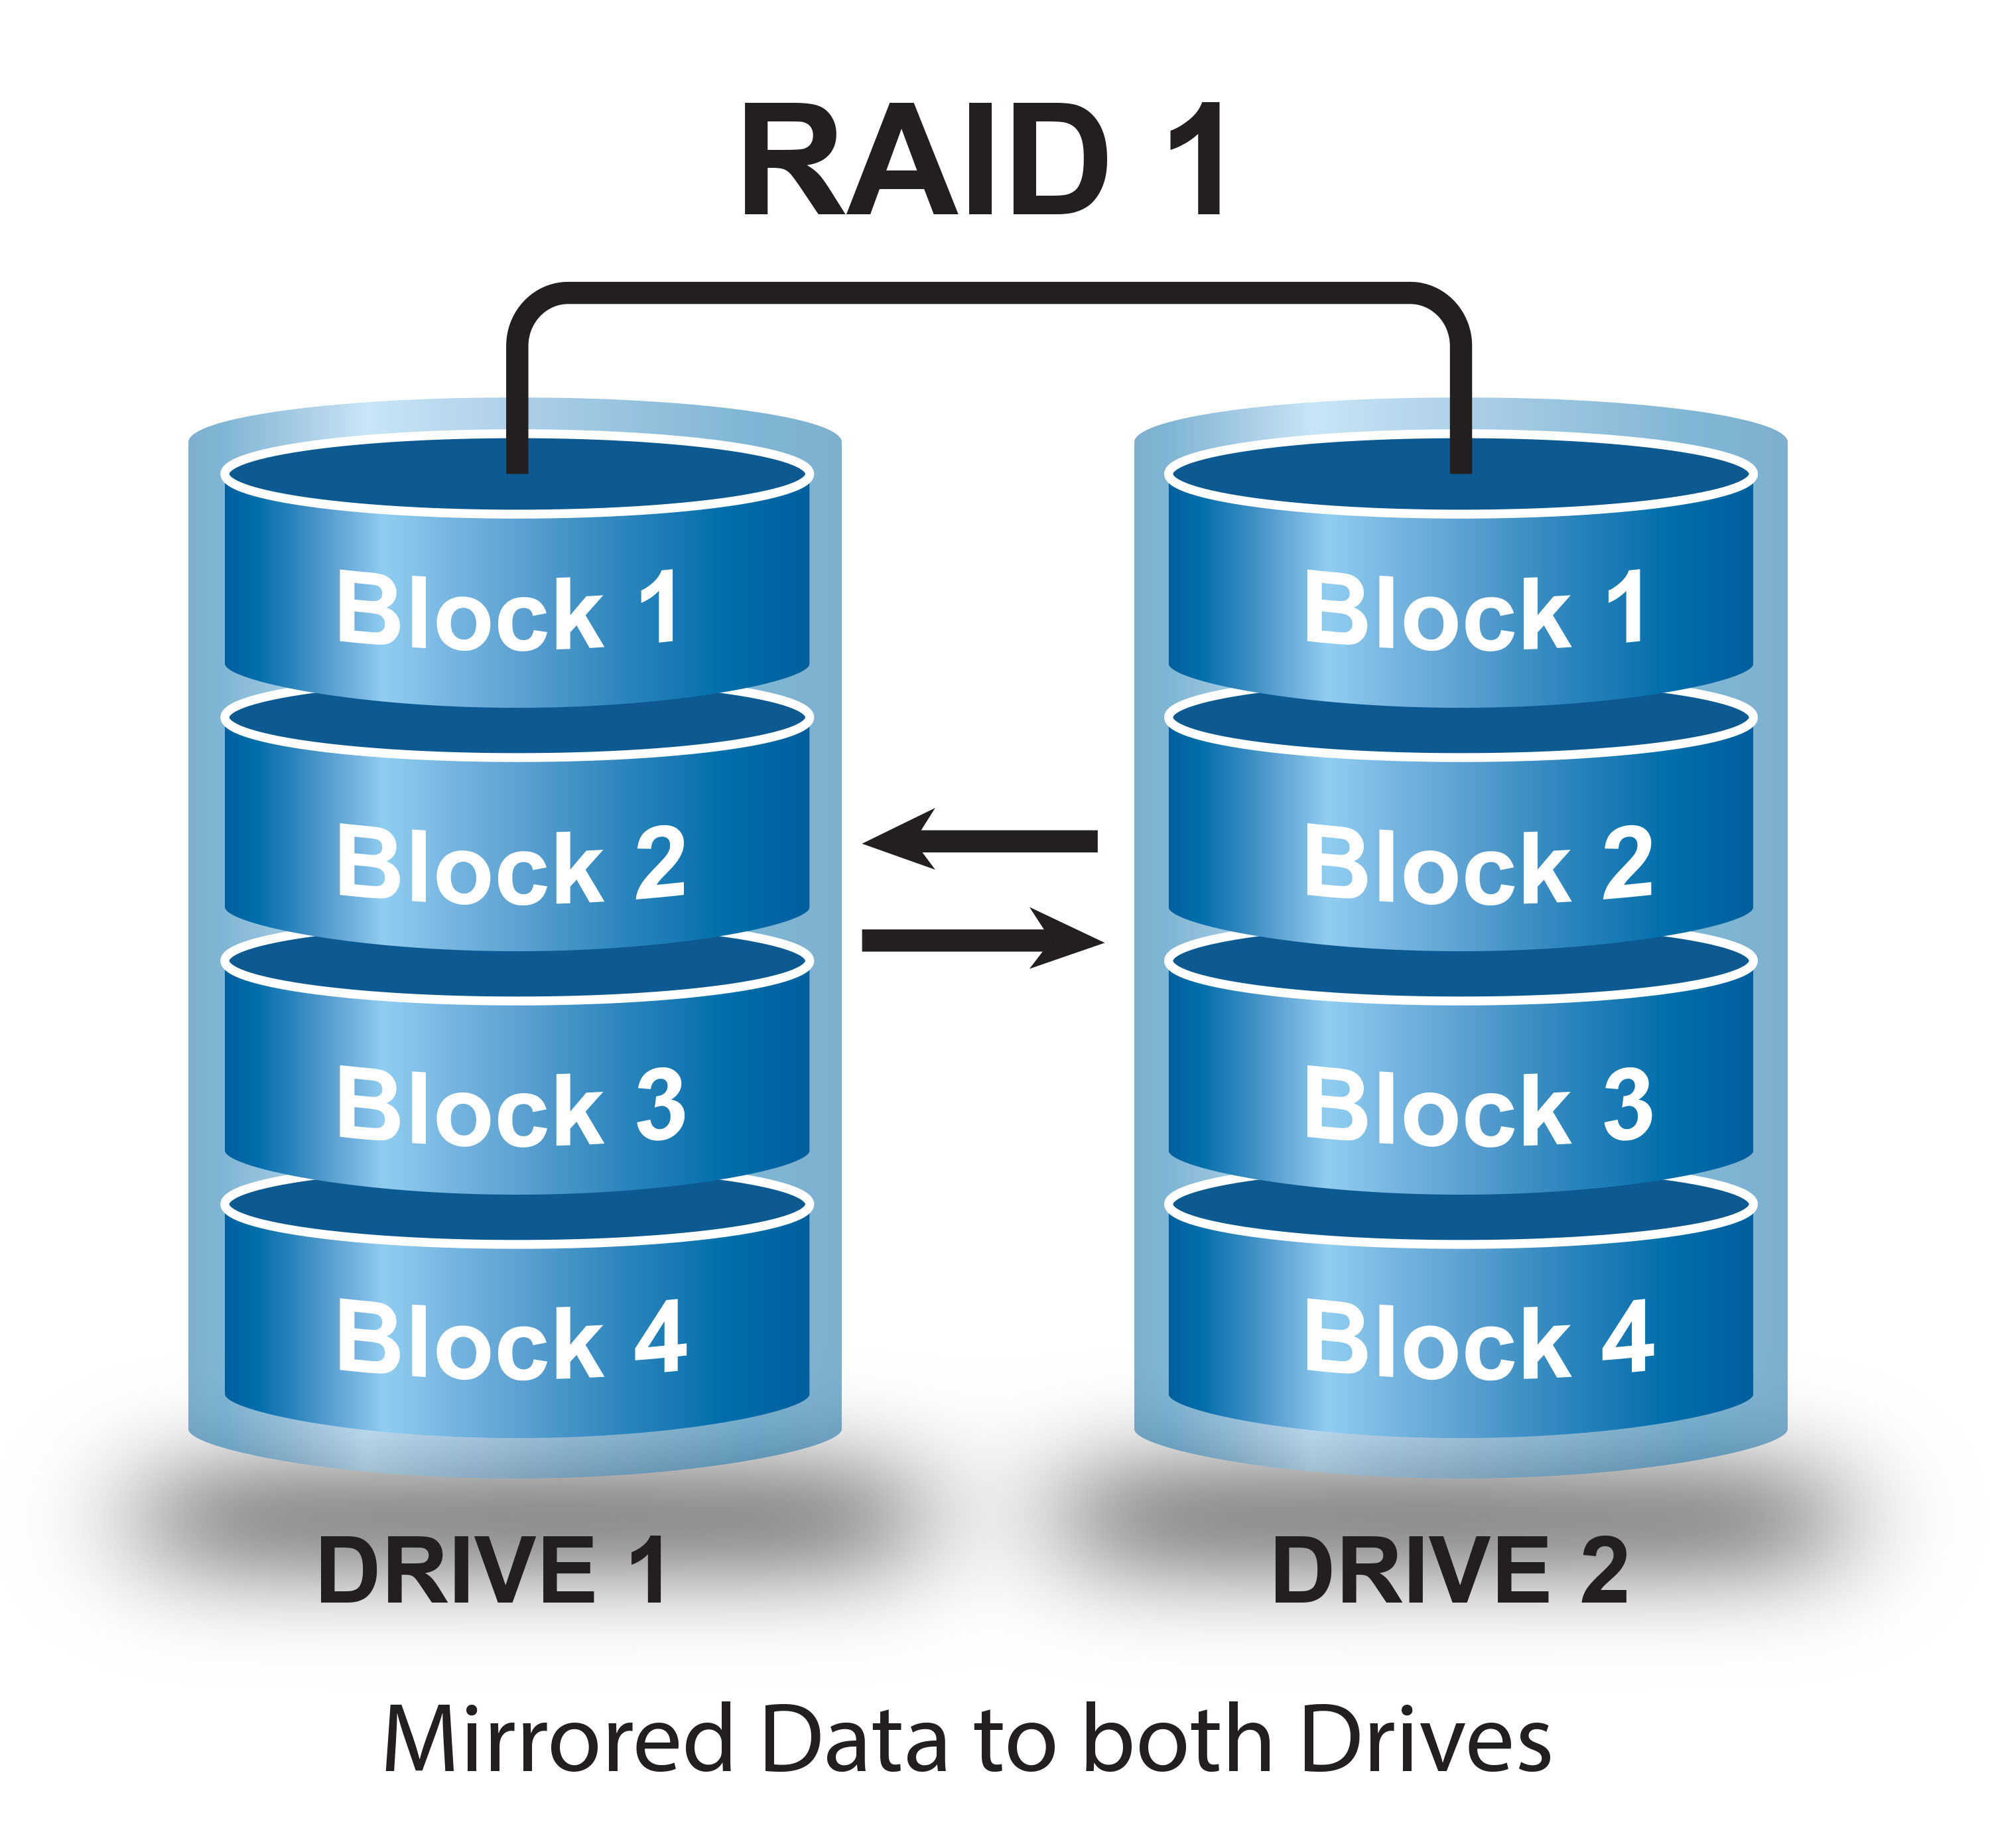
\includegraphics[height=0.7\textheight, keepaspectratio]{../figs/cap08/raid1}
				\end{figure}				
			\end{column}
		\end{columns}	
	\end{frame}	
	
	\begin{frame}[t]{RAID (\textit{Redundant Array of Independent Disks})}{Níveis}
		\begin{itemize}
			\item RAID 2
			\begin{itemize}
				\item Código de correção de erros
				\item Obsoleto
			\end{itemize}	
			\vspace{1em}
			\item RAID 3
			\begin{itemize}
				\item Versão simplificada do RAID2
				\item Obsoleto
			\end{itemize}	
			\vspace{1em}	
			\item RAID 4
			\begin{itemize}
				\item Mínimo de 3 discos
				\item Um disco exclusivo para paridade
			\end{itemize}	
		\end{itemize}
	\end{frame}
	
	\begin{frame}[t]{RAID (\textit{Redundant Array of Independent Disks})}{Níveis}
		\begin{itemize}
			\item RAID 5
			\begin{itemize}
				\item Paridade distribuída
			\end{itemize}
			
					\begin{figure}
		\centering
		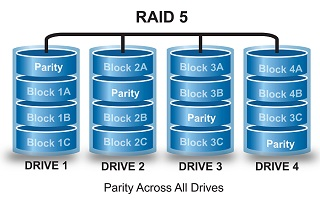
\includegraphics[height=0.7\textheight, keepaspectratio]{../figs/cap08/raid5}
		\end{figure}
		\end{itemize}
		
	\end{frame}	
	
	\section{Discos de Estado Sólido}
	\begin{frame}{Disco de estado sólido}
		\begin{columns}
			\begin{column}{0.5\textwidth}
				\begin{itemize}
					\item \textit{Solid State Disks} - SSD
					\vspace{1em}
					\item Dispositivo de armazenamento não volátil
					\vspace{1em}
					\item Conjunto de memórias semicondutoras
				\end{itemize}
			\end{column}
			\begin{column}{0.5\textwidth}
				\begin{figure}[hbtp]
				\centering
				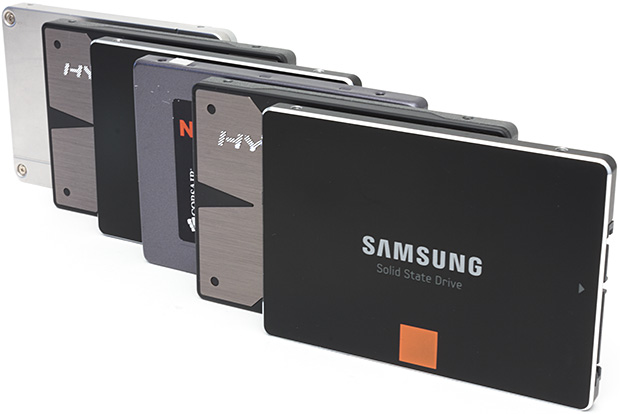
\includegraphics[width=0.8\textwidth, keepaspectratio]{../figs/cap08/ssd.jpg}
				\end{figure}			
			\end{column}
		\end{columns}

	\end{frame}
	
	\begin{frame}{Vantagens}
		\begin{itemize}
			\item Imunidade a falhas devido à vibração e choque físico
			\vspace{1em}
			\item Baixo consumo de energia
			\vspace{1em}
			\item Tamanho reduzido
			\vspace{1em}
			\item Menor peso
		\end{itemize}
	\end{frame}
	
	\begin{frame}{Desvantagens}
		\begin{itemize}
			\item Alto custo por bit (comparado ao armazenamento magnético)
			\vspace{1em}
			\item Limitação de quantidade de operações de escrita
		\end{itemize}
		
		\begin{figure}[hbtp]
		\centering
		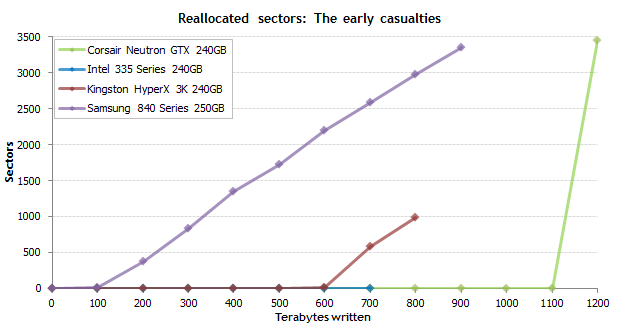
\includegraphics[height=0.6\textheight, keepaspectratio]{../figs/cap08/earlyfailures.png}
		\end{figure}		
	\end{frame}
	
	\begin{frame}{Construção}
		\begin{itemize}
			\item Placa de circuito impresso única
			\begin{itemize}
				\item Conjunto de memórias
				\item Controlador do disco
				\item Alimentação
			\end{itemize}
			
		\end{itemize}
		
		\begin{figure}[hbtp]
		\centering
		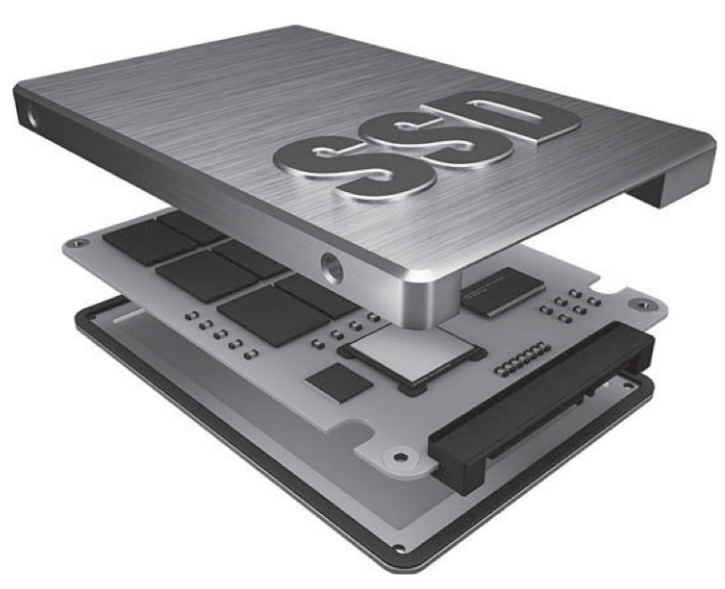
\includegraphics[height=0.4\textheight, keepaspectratio]{../figs/cap08/ssd01.png}
		\end{figure}
		
	\end{frame}

	\begin{frame}{Construção}
	
		\begin{columns}
			\begin{column}{0.5\textwidth}
				\begin{itemize}
					\item Células Flash NAND
					\begin{itemize}
						\item \textit{Single-Level Cell} - SLC
						\item \textit{Multi-Level Cell} - MLC
						\item \textit{Triple-Level Cell} - TLC
					\end{itemize}			
				\end{itemize}
			\end{column}
			\begin{column}{0.5\textwidth}
				\begin{figure}[hbtp]
					\centering
					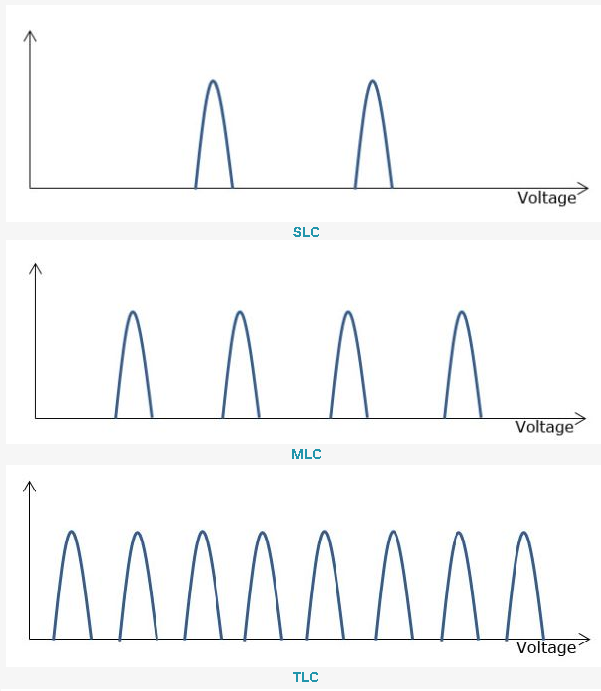
\includegraphics[height=0.8\textheight, keepaspectratio]{../figs/cap08/ssd03.png}
				\end{figure}
			\end{column}
		\end{columns}
		

		
	\end{frame}
	
	\begin{frame}{Construção}
		\begin{figure}[hbtp]
			\centering
			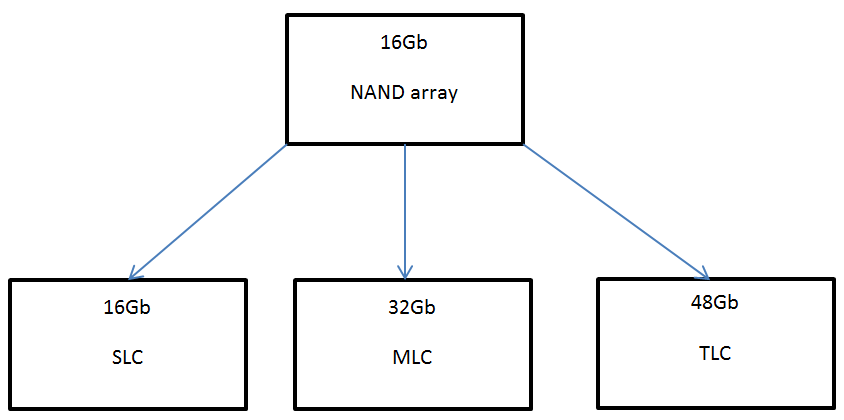
\includegraphics[height=0.75\textheight, keepaspectratio]{../figs/cap08/ssd02.png}
		\end{figure}
	\end{frame}
	
	\begin{frame}{Organização}
		\begin{columns}
			\begin{column}{0.5\textwidth}
				\begin{itemize}
					\item Organização em páginas
					\begin{itemize}
						\item Tamanho padrão: 4 kB
					\end{itemize}
					\vspace{1em}
					\item Páginas agrupadas em blocos
					\begin{itemize}
						\item Tamanho típico: 128 páginas
					\end{itemize}
				\end{itemize}			
			\end{column}
			\begin{column}{0.5\textwidth}
				\begin{figure}[hbtp]
				\centering
				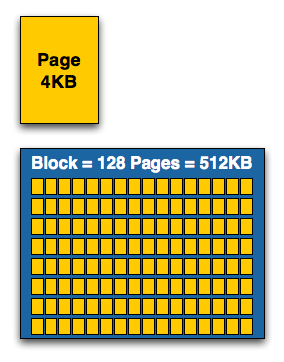
\includegraphics[height=0.8\textheight, keepaspectratio]{../figs/cap08/pageandblock.png}
				\end{figure}
			\end{column}
		\end{columns}

	\end{frame}
	
	\begin{frame}{Organização}
		\begin{itemize}
			\item Painéis
		\end{itemize}
		
		\begin{figure}[hbtp]
		\centering
		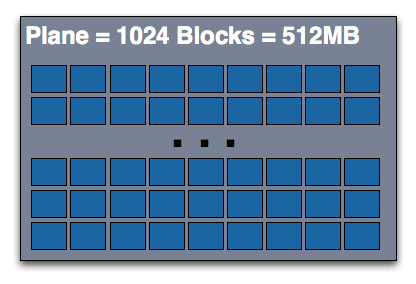
\includegraphics[height=0.75\textheight, keepaspectratio]{../figs/cap08/plane.png}
		\end{figure}		
	\end{frame}
	
	\section{Meios Óticos}
	\begin{frame}{Armazenamento Ótico}
		\begin{itemize}
			\item Armazenamento não volátil
			\vspace{1em}
			\item CD, DVD, Blu-ray
			\vspace{1em}
			\item Capacidade de 700 MB (CD), 4.7 GB (DVD) e 50 GB (Blu-ray)
			\begin{itemize}
				\item Possibilidade de gravação \textit{double-layer} - duplicação da capacidade de armazenamento
			\end{itemize}
		\end{itemize}
		\begin{figure}[hbtp]
		\centering
		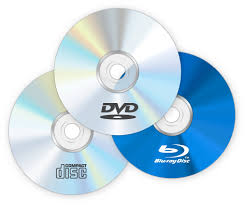
\includegraphics[height=0.25\textheight, keepaspectratio]{../figs/cap08/otico}
		\end{figure}			
	\end{frame}
	
	\begin{frame}{Compact Disk - CD}
		\begin{columns}
			\begin{column}{0.6\textwidth}
		\begin{itemize}
			\item Primeira tecnologia de armazenamento ótico amplamente utilizada
			\vspace{1em}
			\item Capacidade de 700 MB
			\begin{itemize}
				\item 74 minutos de áudio
				\item 20 minutos de vídeo
			\end{itemize}
			\vspace{1em}
			\item Utilização de feixes de luz infravermelha (780 nm)
		\end{itemize}
			\end{column}
			\begin{column}{0.4\textwidth}
		\begin{figure}[hbtp]
		\centering
		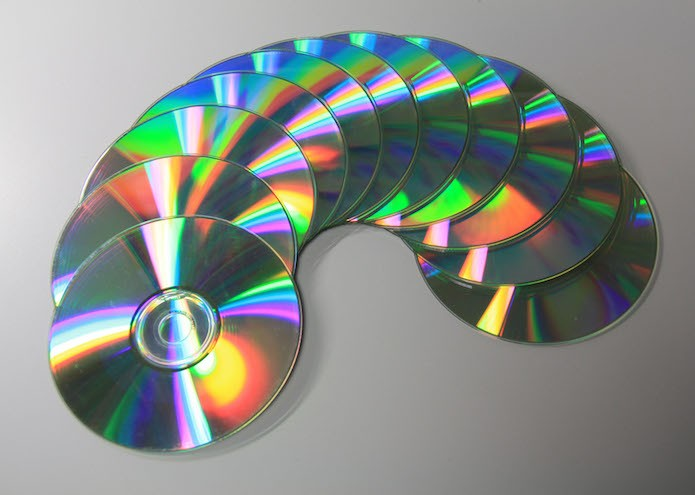
\includegraphics[width=0.75\textwidth, keepaspectratio]{../figs/cap08/cd}
		\end{figure}	
			\end{column}
		\end{columns}
	\end{frame}
	
	\begin{frame}{Organização dos dados}
		\begin{figure}[hbtp]
		\centering
		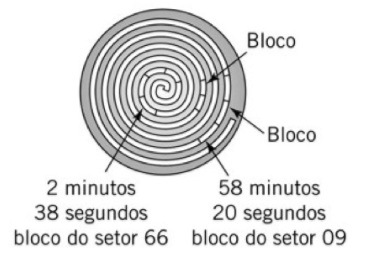
\includegraphics[height=0.85\textheight, keepaspectratio]{../figs/cap08/cdblock}
		\end{figure}		
	\end{frame}
	
	\begin{frame}{Organização dos dados}
		\begin{itemize}
			\item 270 mil blocos
			\vspace{1em}
			\item Capacidade do bloco
			\begin{itemize}
				\item 2352 bytes de extensão
				\item 2048 bytes de dados
				\item 16 bytes de cabeçalho
				\item 288 bytes de correção de erros (Reed Solomon)
			\end{itemize}
			\vspace{1em}
			\item Identificação do bloco
			\begin{itemize}
				\item Ocupa 4 bytes do cabeçalho
				\item 3 bytes indicam o setor, minuto e segundo
				\item 1 byte de modo de operação
			\end{itemize}
		\end{itemize}
	\end{frame}
	
	\begin{frame}{Organização dos dados}
		\begin{figure}[hbtp]
		\centering
		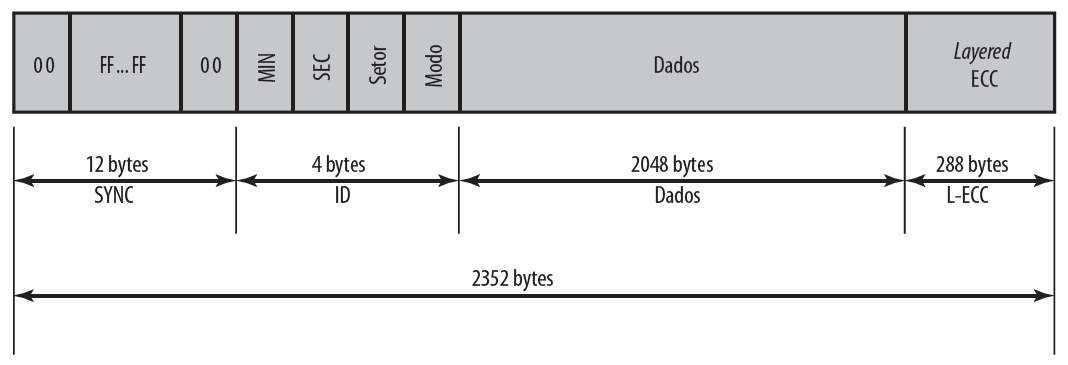
\includegraphics[width=0.95\textwidth, keepaspectratio]{../figs/cap08/organizacaoCD}
		\caption{Formato de bloco de CD-ROM }
		\end{figure}		
	\end{frame}

	\begin{frame}{Armazenamento}
		\begin{columns}
			\begin{column}{0.5\textwidth}
				\begin{itemize}
					\item Reentrâncias (\textit{lands}) 
					\item Saliências (\textit{pits})
				\end{itemize}
				\begin{figure}[hbtp]
				\centering
				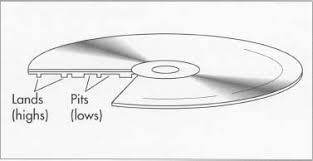
\includegraphics[width=0.85\textwidth, keepaspectratio]{../figs/cap08/landpit}
				\end{figure}				
			\end{column}
			\begin{column}{0.5\textwidth}
				\begin{figure}[hbtp]
				\centering
				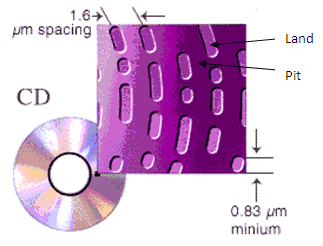
\includegraphics[width=0.85\textwidth, keepaspectratio]{../figs/cap08/landpit2}
				\end{figure}
			\end{column}
		\end{columns}

	\end{frame}
	
	\begin{frame}{Escrita de dados}
		\begin{columns}
			\begin{column}{0.5\textwidth}
		\begin{itemize}
			\item Modificação do padrão de \textit{lands} e \textit{pits}
			\vspace{1em}
			\item Utilização de um laser especial para escrita (\textit{Write Laser})
			\vspace{1em}
			\item Laser cria uma série de \textit{pits}
		\end{itemize}			
			\end{column}
			\begin{column}{0.5\textwidth}
		\begin{figure}[hbtp]
			\centering
			
\includegraphics[width=0.7\textwidth, keepaspectratio]{../figs/cap08/cdburn}
		\end{figure}			
			\end{column}
		\end{columns}
	\end{frame}
	
	\begin{frame}{Leitura de dados}
		\begin{figure}[hbtp]
			\centering
			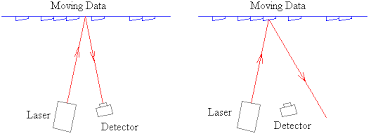
\includegraphics[width=0.9\textwidth, keepaspectratio]{../figs/cap08/cdreading}
		\end{figure}			
	\end{frame}
	
	\begin{frame}{Leitura dos dados}
		\begin{figure}[hbtp]
		\centering
		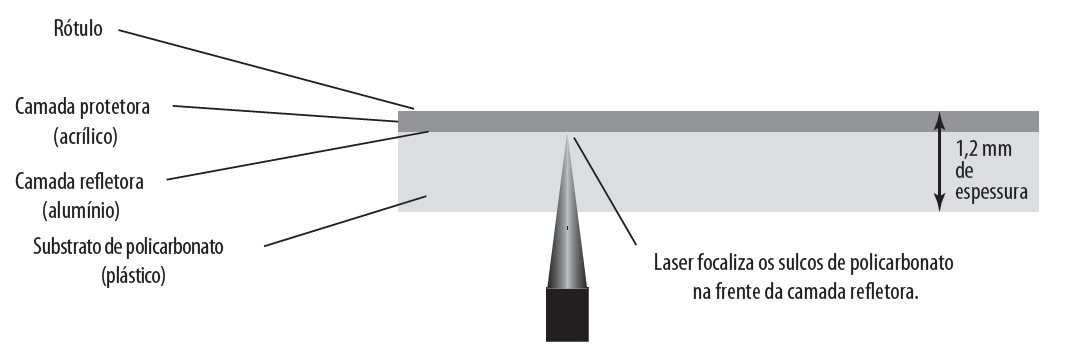
\includegraphics[width=0.95\textwidth, keepaspectratio]{../figs/cap08/cd1}
		\end{figure}		
	\end{frame}
		
	\begin{frame}{Digital Versatile Disc - DVD}
		\begin{itemize}
			\item Aumento da capacidade de armazenamento - 4.7 GB
			\vspace{1em}
			\item Possibilidade de gravação em duas camadas (\textit{double layer})
			\begin{itemize}
				\item Capacidade de 8.6 GB
			\end{itemize}
			\vspace{1em}
			\item Feixe de luz vermelha (650nm)
		\end{itemize}
	\end{frame}
	
	\begin{frame}{Organização dos dados}
		\begin{figure}[hbtp]
			\centering
			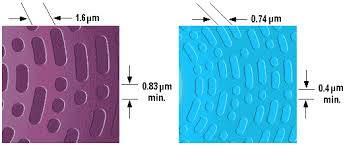
\includegraphics[width=0.9\textwidth, keepaspectratio]{../figs/cap08/cddvd}
		\end{figure}			
	\end{frame}
	
	\begin{frame}{Formatos}
		\begin{eftable}
			\centering
			\begin{tabular}{c|c|c}
				\textcolor{white}{Número de faces} & 
				\textcolor{white}{Número de camadas} & 
				\textcolor{white}{Capacidade de armazenamento} \\ 
				1 & 1 & 4,7 GB \\ 
				1 & 2 & 8,6 GB \\ 
				2 & 1 & 9,4 GB \\ 
				2 & 2 & 17 GB \\ 
			\end{tabular} 
		
		\end{eftable}
	\end{frame}

	\begin{frame}{Leitura de dados}
		\begin{figure}[hbtp]
			\centering
			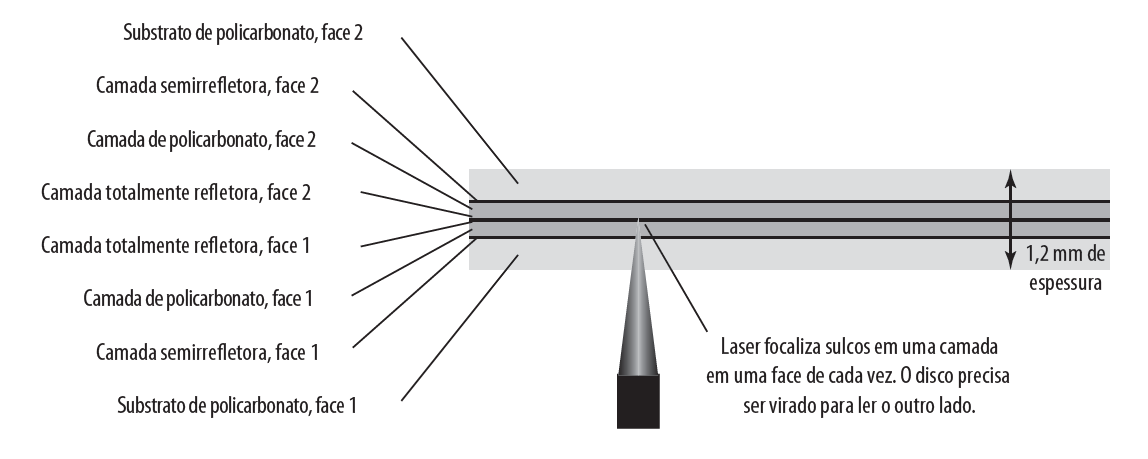
\includegraphics[width=\textwidth, keepaspectratio]{../figs/cap08/dvd}
		\end{figure}			
	\end{frame}
	
	\begin{frame}{Blu-ray Disc - BD}		
		\begin{columns}
			\begin{column}{0.6\textwidth}
				\begin{itemize}
					\item Capacidade de armazenamento de 25 GB
					\vspace{1em}
					\item Feixe de luz azul (406 nm)
				\end{itemize}
			\end{column}
			\begin{column}{0.4\textwidth}
		\begin{figure}[hbtp]
			\centering
			
\includegraphics[width=\textwidth, keepaspectratio]{../figs/cap08/bluray}
		\end{figure}
			\end{column}
		\end{columns}

		
	\end{frame}

	\begin{frame}{Armazenamento de Dados}
		\begin{figure}[hbtp]
			\centering
			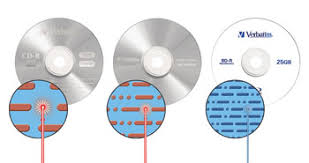
\includegraphics[height=0.75\textheight, keepaspectratio]{../figs/cap08/otico4}
		\end{figure}
	\end{frame}
	
	\begin{frame}{Comparativo}
				\begin{figure}[hbtp]
			\centering
			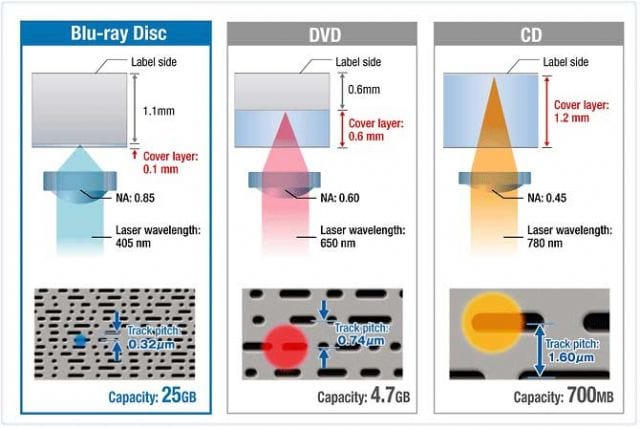
\includegraphics[height=0.8\textheight, keepaspectratio]{../figs/cap08/otico2}
		\end{figure}
	\end{frame}
	
	\begin{frame}{Comparativo}
				\begin{figure}[hbtp]
			\centering
			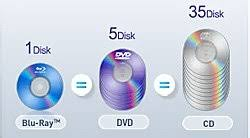
\includegraphics[width=0.7\textwidth, keepaspectratio]{../figs/cap08/otico3}
		\end{figure}
	\end{frame}
	
%	\section{Memória Virtual}

	\section{Referências}
	\begin{frame}{Bibliografia}
		\nocite{Englander2011}
		\nocite{Monteiro2010}
		\nocite{Stallings2010}
		\nocite{Vatto2012}
		\nocite{Tanenbaum2007}
    	\bibliographystyle{ieeetr}
    	\bibliography{../refs}
    	
	
	\end{frame}

\end{document}
